\chapter{BG}
\section{Arificial neural network (ANN)}
Arificial neural networks are inspired by the mechanisms of human brain. Human neuron cells are in ANN replaced replaced by artificial neurons, which are difined as:
\begin{align}
    y = f \left( \boldsymbol{w}^T \boldsymbol{x}  + b \right).
\end{align}
Where $\boldsymbol{x}$ is vector of inptus, $\boldsymbol{w}$ are weights and $b$ is bias. Symbol $f$ denotes an activation funtion f : $\mathbb{R} \rightarrow \mathbb{R}$. The artificial neuron proposed by Frank Rosenblatt in the perceptron algorithm used step funtion \cite{Rosenblatt1958}, but nowadays different functions such as ReLu, sigmoid or tanh are used. Output of the neuron $y$ is called activation of the neuron.

Neurons are ussally structured into layers. The connection between layers is depended upon the architecture choice. First ANN used fully connected layers, meaning that the input input a nuron in layer $n$ were all activation from layer $n_1$. Fully connected neural networks are nowdays sparsely used in computer vision and convolutional neural networks (CNNs) are used instead. In case of CNNs we limit the receptive field of neuron to local neighborhood only, this decreases the computation complexity and includes our prior knowledge of pixel neighborhood in input image. Having the same weights for whole input makes the network invariant to shifts in the input.

\section{Convolutional layer}
Convolutional layers consists of $C_{out}$ neurons, each having $C_{in}, H, W$ receptive field. Those neurons ale called kernels with width $W$ height $H$ and number of input channels $C_{in}$. In each layer we convolve\footnote{Even though we usually refer to convolution, in practice cross-corelation is used instead and terms cross-corelation and convolution are used interchangebly.} the input $X$  with the kernel $W$, the output $Y$ is defined by:
\begin{align}
    y_{o,i,j} = \sum_{c_{in}} \sum_{\Delta i} \sum_{\Delta j} x_{c, i+\Delta i, j + \Delta j}  w_{o,c, \Delta i, \Delta j}
\end{align}
Nowadays modifications of convolutional layers are proposed, such as dilated convolution, gruped convolution or depth-wise seprable convolutions are proposed, but the fundamentals are the same: Filter sliding over the input producing an output.


\begin{figure}
    \centering
    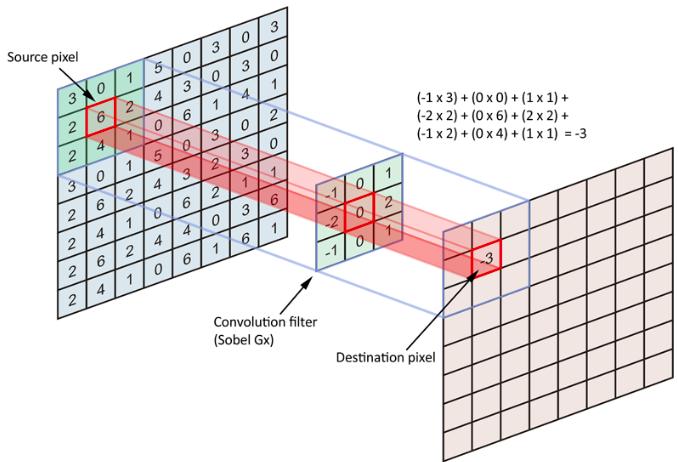
\includegraphics[width=0.9\linewidth]{images/conv_img.png}
\end{figure}

\section{Activation functions}
Output of convolutional layer is usually folowed by non-linear activation function. Many activation function are at our disposal, but the most commonly used is ReLU and its derivatives such as: SERLU, SELU, ELU, Swish, Leaky ReLU. Values of those function are depicted in figure \ref{fig:activation_functions}.

\begin{figure}
    \centering
    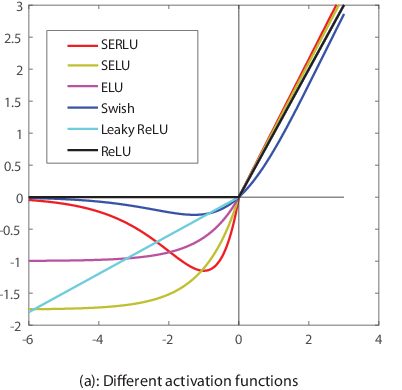
\includegraphics[width=0.6\linewidth]{images/activation_functions.png}
    \caption{Graphs of ReLU based activation functions, source \cite{Zhang2018}}
    \label{fig:activation_functions}
\end{figure}

\section{Batch-normalization and it derivatives}
\subsection{Batch-normalization}


\section{Transformer architecture}
Transformer architecture debuted in the field of computer vison in 2021 and since then achieved great results, beating state of the art models in multiple benchmarks across all computer vision tasks. As of May 2022, the best performing models in the main computer vision benchmarks are based on transformer architecture. We think of the following benchmarks to be the main ones in computer vision:  ImageNet benchmark (classification task), COCO (object detection), ADE20K (semantic segmentation).

The transformer architecture was proposed already in 2017 for the task of nature language processing (NLP), we will briefly introduce transformer architectire for the NLP task, since it is crucial for understanding of transformers for computer vison.

\subsubsection{Transformers in NLP}
Transformer architecture was introduced in paper Attention is all you need \cite{Vaswani2017} for the purpose of NLP. NLP is task, where input is a sequence of words of length $n$ and output is sequence of $m$ words, where $n$ and $m$ usualy differs. Sequence of words is converted into sequence of vectors, there are multuple options how to embed words into vector, commonly used is TD-IDF or Word2Vec\cite{Li2018}. Positional encoding is added to those vector and than processed by encoder block. The novel key layer is self-attention, where for input sequence of vector values $V$, keys $K$ and queries $Q$ are computed. From encoder we output values and keys and from decoder's self-attention module we output queries. We than take keys and values from encoder and queries form decoder and input the into another attention block:
\begin{align}
    Attention \left(Q,K,V \right) = \text{softmax} \left( \frac{QK^T}{\sqrt{d_k}} \right)V,
\end{align}
where $d_k$ is dimension of keys. More details can be seen in figure \ref{fig:nlp_transformer} or in \cite{Vaswani2017}.

\begin{figure}
    \centering
    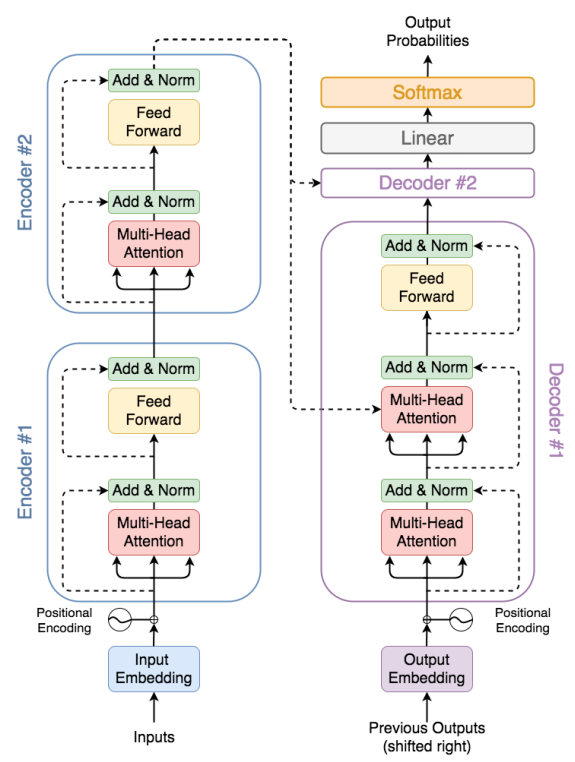
\includegraphics[width=\linewidth]{images/two_layer_transformer.png}
    \caption{Architecure of transformer with two encoders and two decoders, source \cite{Yin2020}}
    \label{fig:nlp_transformer}
\end{figure}

\section{General architecture for object detection}
Even thought, there is broad variety of architectures for object detection, the core principles remains the same. The model is composed from three main parts: backbone, neck, head as shown in figure \ref{fig:object_detection_architecture}. Each of those blocks can useally be swaped for different one, which is fullfiling the same purpose. This gives us great flexibility and allows us to try different combinations of those blocks.

\subsection{Transformers in computer vision}
The first trasnformer based model was Vision Transformer (ViT). It was capable of image classification only and it is composed of multiple encoder blocks stacked on top of each other. Those blocks are same as those used NLP task. On top encoder blocks is attached multi-layer perceptron (MLP) head, which outputs values for each class. Those can be converted into corresponding probabilities by softmax-layer. Input into ViT are $16 \times 16$ image patches lineary projected into vectors, the whole architecture is shown in figure
\begin{figure}
    \centering
    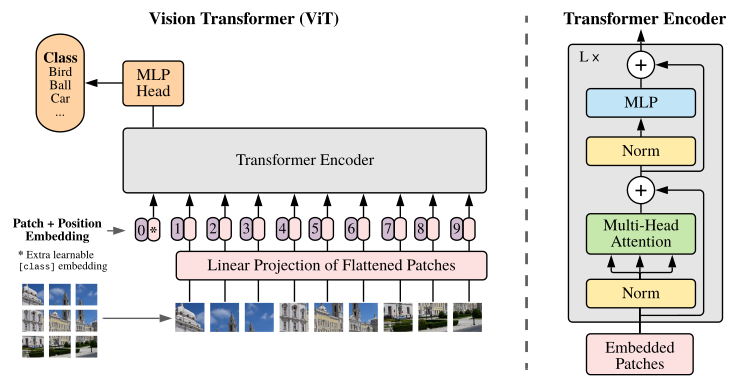
\includegraphics{images/vision_transformer.png}
    \caption{Architecture of ViT, source \cite{Dosovitskiy2020}}
    \label{fig:vision_transformer}
\end{figure}


\begin{figure}
    \centering
    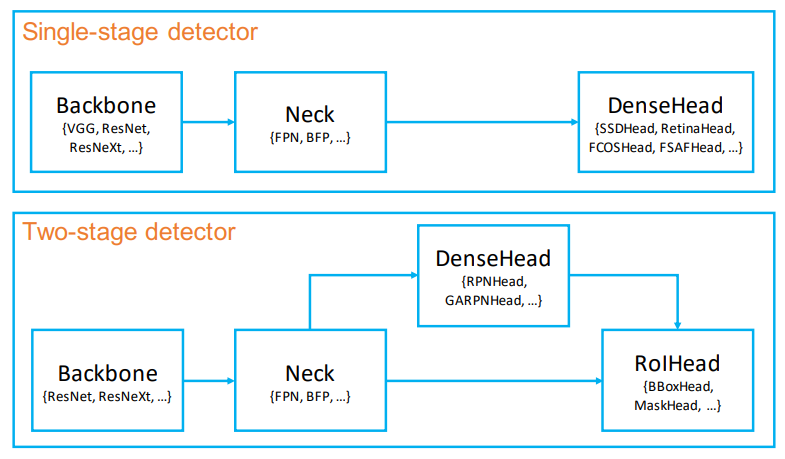
\includegraphics[width=0.6\linewidth]{images/object_detection_architecture.png}
    \caption{General architecture for object detection, source \cite{Chen2019}}
    \label{fig:object_detection_architecture}
\end{figure}

\subsubsection{Backbone}
The purpose of bacbkones is transformation of input image into feature maps. For this purpose are used classification models with classification head removed. Most parameters of object detection models are usually part of the backbone and extracting usefull feature maps is vital for other blocks to perform well. The most common backbones are models from the ResNet family.

\subsubsection{Neck}
Neck is responsible for merging of features from the backbone. This is not straight-forward task, since we usually use features from different layers of the backbone. This allows us to get semanticaly strong features from deeper layers as well as more detailed information from earlier ones. Common neck architectures are feature pyramid network or PANet.

\subsubsection{Head}

\section{Classification models}
\subsection{ResNet}
ResNet architecture was introduced by He et al. \cite{He2015} and proposed a novel element of deep-learning architectures - identity shortcut connection, sometimes called as skip-connection. Let $\mathbf{x}$ be an input into a block, composed of multiple convolutional layers with activation functions in between\footnote{Addition of batch-normalization, or other layers is possible}, we will call this block a mapping $\mathcal{F}$. Output of residual block $\mathcal{H}$, derived from $\mathcal{F}$ is defined as:

\begin{align}
    \mathcal{H}\left(\mathbf{x}\right) = \mathcal{F} \left(\mathbf{x}\right) + \mathbf{x}.
\end{align}
The reasoning behind residual block, is to make it easier to learn identity mapping, if desired. This had other benefits especialy improvment of gradient flow during back-progation, making it ultimatelly easier to optimize such blocks. This ease of optimization can be seen by inspecting loss function landscape of model with and without skip-connections, figure \ref{fig:resnet_loss}.
Final ResNet architecture is composed of multiple residual blocks stack one after other, the models vary in number of layers used, this is denoted in the name with a number such as ResNet50 or ResNet101.

\begin{figure}
    \centering
    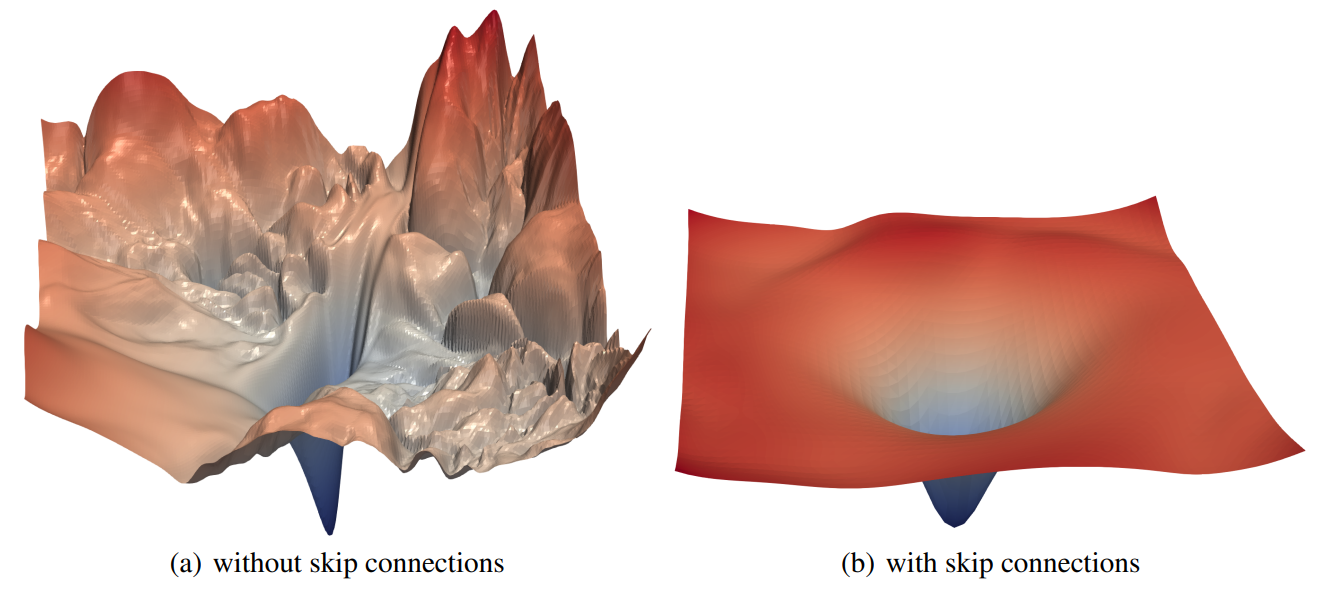
\includegraphics[width=\linewidth]{images/resnet_loss.png}
    \caption{Comparison of loss landscapes, source \cite{Li2017}}
    \label{fig:resnet_loss}
\end{figure}

\subsection{EfficientNet}
When scaling model size we can increase: Number of layers (depth), number of filters in each layer (width) or the width and height of feature maps (resolution). I has been common practice to change only one of them. Tan and Le \cite{Tan2019a} did multi-objective neural network search, where they tried to maximize objective function $O$ defined as:
\begin{align}
    O = ACC \left( m \right) \times \left[ FLOPS \left(m \right) / T \right] ^w,
\end{align}
where $ACC(m)$ and $FLOPS(m)$ are accuracy and FLOPS of model $m$, $T$ is target number of FLOPS and $w$ is a hyper-paremter controling the trade-off between accuracy and number of FLOPS of the final model. From this search resulted the EfficientNet-B0 baseline model, which can be scaled to achieve a bigger network, those are called B1-B7.

\subsection{Swin transformer}
Swin transformer architecture overcomes limitations of ViT, which is working with $16 \times 16$. This is insuficient for task as segmentation and object detection, where dense predictions are needed. Swin transformers are in first layer working with $4 \times 4$ patches. Since computation complexity of self-attention layer grows quadraticaly with number of input tokens, the authors over-come this by ussage of neighbor pathces only. Attention is thus computed with respect to tokens in non-overlaping local window. This local window for computing  self-attention is shifted after every encoder layer as depicted in figure \ref{fig:swin_pathces}. This shift introduces cross-window connections, which increaes modeling capacity of the model. After particular number of encoder layers, neighbor patches are merged. This reduces number of patches, while increasing their size by predefined factor. This mimics the bahaviour of CNNs, where we start with big, semanticaly weak feature maps and gradualy decrease their dimensions, while increasing their number. Having this kind of feature maps allows use to use swin transformer as a general backbone for any task. \cite{Liu2021}

\begin{figure}
    \begin{floatrow}[2]
        \ffigbox[\FBwidth]{\caption{Hierachical structure of Swin Transformer compared with ViT, source \cite{Liu2021}}\label{fig:swin_hierarchy}}%
        {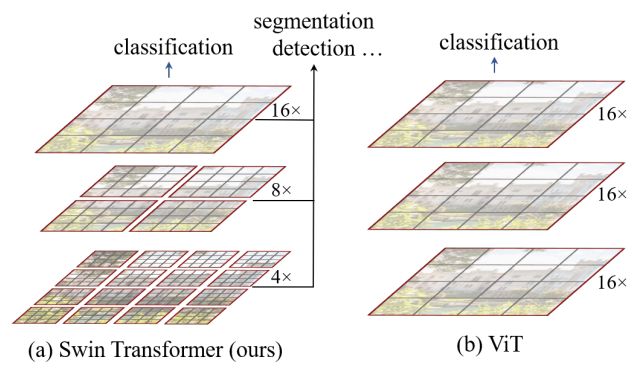
\includegraphics[width=\linewidth]{images/swint_transformer_hierarchy.png}}\qquad
        \ffigbox[\FBwidth]{\caption{Shift of local window for computation of self-attention, source \cite{Liu2021}}\label{fig:swin_pathces}}%
        {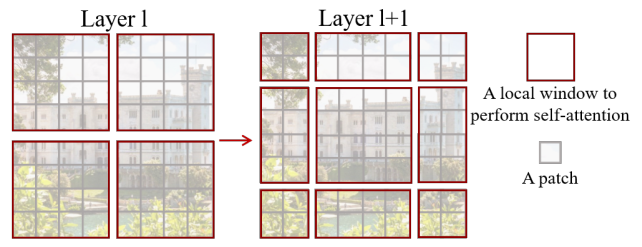
\includegraphics[width=\linewidth]{images/swint_transformer_patches.png}}
    \end{floatrow}
\end{figure}

\section{Detection models}

\subsection{RCNN, Fast-RCNN, Faster-RCNN}

\subsection{RetinaNet}

\subsection{YOLO family}

\subsection{EfficientDet}